\documentclass[english,9pt,aspectraio=169]{beamer}
\usepackage{etex}
\usetheme{uzhneu-en-informal}
%\usepackage{uarial}
\usepackage[T1]{fontenc}
\usepackage[utf8]{inputenc}
\RequirePackage{graphicx,ae}
\usepackage{bm}
\usepackage{fancybox,amssymb,color}
\usepackage{pgfpages}
\usepackage{booktabs}
\usepackage{verbatim}
\usepackage{animate}
\usepackage{numprint}
\usepackage{dsfont}
\usepackage{tikz}
\usepackage{amsmath,natbib}
\usepackage{mathbbol}
\usepackage{babel}
\usepackage{SweaveSlides}
\usepackage{multicol}
\usepackage{xcolor}


\usetheme{uzhneu-en-informal}
\DeclareMathOperator{\po}{Poisson}
\DeclareMathOperator{\G}{Gamma}
\DeclareMathOperator{\Be}{Beta}
\DeclareMathOperator{\logit}{logit}
\def\n{\mathop{\mathcal N}}

\definecolor{Gray}{RGB}{139,137,137}
\definecolor{darkred}{rgb}{0.8,0,0}
\definecolor{Green}{rgb}{0,0.8,0.3}
\definecolor{Blue}{rgb}{0,0,1}
\def\myalert{\textcolor{darkred}}
\def\myref{\textcolor{Gray}}
\setbeamercovered{invisible}

\renewcommand{\baselinestretch}{1.2}
\beamertemplateballitem
\DeclareMathOperator{\cn}{cn} % Copy number
\DeclareMathOperator{\ccn}{ccn} % common copy number
\DeclareMathOperator{\p}{p} % common copy number
\DeclareMathOperator{\E}{E} % common copy number
\DeclareMathOperator{\given}{|} % common copy number
\def\given{\,|\,}
\def\na{\tt{NA}}
\def\nin{\noindent}
\pdfpageattr{/Group <</S /Transparency /I true /CS /DeviceRGB>>}
\def\eps{\varepsilon}

\renewcommand{\P}{\operatorname{\mathsf{Pr}}} % Wahrscheinlichkeitsmaß
\def\eps{\varepsilon}
\def\logit{\text{logit}}
%\newcommand{\E}{\mathsf{E}} % Erwartungswert
\newcommand{\Var}{\text{Var}} % Varianz
\newcommand{\NBin}{\text{NBin}}
\newcommand{\Po}{\text{Po}}
\newcommand{\N}{\mathsf{N}}

\newcommand{\ball}[1]{\begin{pgfpicture}{-1ex}{-0.65ex}{1ex}{1ex}
\usebeamercolor[fg]{item projected}

{\pgftransformscale{1.75}\pgftext{\normalsize\pgfuseshading{bigsphere}}}
{\pgftransformshift{\pgfpoint{0pt}{0.5pt}}
\pgftext{\usebeamerfont*{item projected}{#1}}}
\end{pgfpicture}}%
\usepackage{multicol}
\newcommand{\ballsmall}[1]{\begin{pgfpicture}{-1ex}{-0.65ex}{.2ex}{.2ex}

{\pgftransformscale{1}\pgftext{\normalsize\pgfuseshading{bigsphere}}}
{\pgftransformshift{\pgfpoint{0pt}{0.5pt}}
\pgftext{\usebeamerfont*{item projected}{#1}}}
\end{pgfpicture}}%




\begin{document}

\fboxsep5pt

\frame{
\title[]{ \centering \Huge Kurs Bio144: \\
Datenanalyse in der Biologie}%\\[.3cm]
\author[Stefanie Muff, Owen L.\ Petchey]{\centering Stefanie Muff  \& Owen L.\ Petchey }
%\institute[]{Institute of Social and Preventive Medicine \\ Institute of Evolutionary Biology and Environmental Studies}
\date[]{Week 4: Multiple linear regression (finalize) / Residual analysis / Checking modelling assumptions\\ 16./17. March 2017}


\maketitle
}


\frame{\frametitle{Overview (todo: check)}
\begin{itemize}
\item Interactions between covariates
\item Multiple vs.\ many single regressions
\item Checking assumptions / Model validation 
\item What to do when things go wrong?
\item Transformation of variables/the response
\item Handling of outliers
\end{itemize}
}


\frame{\frametitle{Course material covered today}
\begin{itemize}
\item Chapter 3.3 in \emph{Lineare Regression}
\item To do
\end{itemize}
}

\frame[containsverbatim]{\frametitle{Recap of last week I}
to do 
}

\frame[containsverbatim]{\frametitle{Recap of last week I}
Last week we introduced binary and factor covariates that allowed for group-specific intercepts.
}


\frame[containsverbatim]{\frametitle{Group-specific slopes / Interactions}
It may happen that groups do not only differ in their intercept ($\beta_0$), but also in their slopes ($\beta_x$).\\[2mm]

For simplicity, let us look at a binary covariate ($x_i \in \{0,1\}$). 
}



\frame[containsverbatim]{\frametitle{}

Remember the mercury (Hg) example from last week. We now extended the dataset and include mothers \emph{and} children ($\leq 11$ years).\\[2mm]

It is known that Hg concentrations may change over the lifetime of humans. So let us look at \texttt{log(Hg$_\text{urin}$)} depending on the participants age:
\vspace{-5mm}
\begin{center}
\setkeys{Gin}{width=0.55\textwidth}
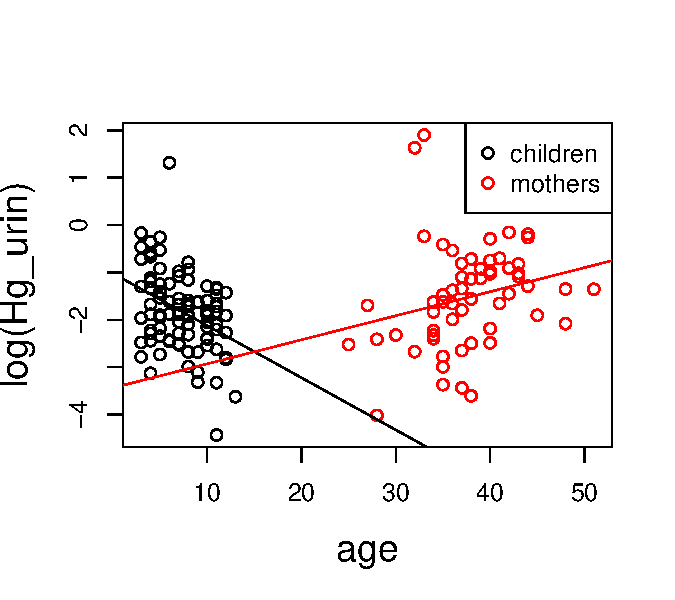
\includegraphics{Bio144_2017_week4-001}
\end{center}
An important observation is that children and mothers show different dependencies of age!
}

\frame{
It is therefore crucial to formulate a model that allows for different intercepts \emph{and} slopes, depending on group membership (mother/child).\\[2mm]

The smallest possible model is then given as\\
\begin{equation}\label{eq:HgInt}
y_i =  \beta_0 + \beta_1 \text{mother}_i + \beta_2 \text{age}_i + \beta_3\text{age}_i\cdot \text{mother}_i + e_i \ , 
\end{equation}
~\\
where $y_i=\log(Hg_{\text{urin}})_i$, and \texttt{mother} is a binary ``dummy'' variable that indicates if the person is a mother (1) or a child (0).\\[4mm]

This results in essentially {\bf two} models with group specific intercept and slope:\\[2mm]
\colorbox{lightgray}{\begin{minipage}{10cm}
Mothers ($x_i=1$): $\hat{y}_i = \beta_0 +  \beta_1 + (\beta_2 +\beta_3)\text{age}_i + e_i$  \\[2mm]
Children ($x_i=0$): $\hat{y}_i = \beta_0  + \beta_2 \text{age}_i + e_i$  
\end{minipage}}
}




\frame[containsverbatim]{\frametitle{}
Fitting model \eqref{eq:HgInt} in R is done as follows, where \texttt{age:mother} denotes the interaction term ($\text{age}_i\cdot \text{mother}_i$):\\[6mm]

\begin{Schunk}
\begin{Sinput}
> r.hg <- lm(log(Hg_urin)~  mother + age + age:mother,d.hg)
> summary(r.hg)$coef
\end{Sinput}
\begin{Soutput}
              Estimate Std. Error   t value     Pr(>|t|)
(Intercept) -1.0188317 0.25250071 -4.034966 8.624100e-05
mother      -2.4176907 0.91198012 -2.651034 8.874694e-03
age         -0.1101447 0.03225589 -3.414715 8.188542e-04
mother:age   0.1609032 0.03965739  4.057333 7.912112e-05
\end{Soutput}
\end{Schunk}
~\\[4mm]

Interpretation: \\[2mm]

Mothers: $\hat{y}_i = -1.02 + (-2.42) + (-0.11 + 0.16) \cdot \text{age}_i$ \\[2mm]
Children: $\hat{y}_i = -1.02  + (-0.11) \cdot \text{age}$ \\[2mm]

\begin{itemize}
\item The Hg level drops in young children.
\item The Hg level increases in adults (mothers).
\end{itemize}
}

\frame[containsverbatim]{\frametitle{}
Remember (from last week), however, that the Hg model also included smoking status, amalgam fillings and fish consumption as important predictors. It is very straightforward to just include these predictors in model \eqref{eq:HgInt}, which leads to the following model \\[6mm]

\begin{Schunk}
\begin{Sinput}
> r.hg <- lm(log(Hg_urin)~  mother * age + smoking + amalgam + fish,d.hg)
\end{Sinput}
\end{Schunk}

% latex table generated in R 3.3.2 by xtable 1.8-2 package
% Wed Nov  2 20:44:56 2016
\begin{table}[!h]
\centering
\begingroup\footnotesize
\begin{tabular}{rrrr}
  \hline
 & Coefficent & 95\%-confidence interval & $p$-value \\ 
  \hline
Intercept & -1.35 & from -1.82 to -0.87 & $<$ 0.0001 \\ 
  mother & -2.66 & from -4.38 to -0.94 & 0.003 \\ 
  age & -0.098 & from -0.16 to -0.04 & 0.001 \\ 
  smoking & 0.60 & from 0.06 to 1.15 & 0.03 \\ 
  amalgam & 0.19 & from 0.10 to 0.28 & $<$ 0.0001 \\ 
  fish & 0.072 & from 0.04 to 0.10 & $<$ 0.0001 \\ 
  mother:age & 0.14 & from 0.07 to 0.22 & 0.0001 \\ 
   \hline
\end{tabular}
\endgroup
\end{table}
{\small (Note that \texttt{mother*age} in R encodes for \texttt{mother} + \texttt{age} + \texttt{mother:age}.)}
}

\frame[containsverbatim]{
Again, for completeness, some model checking: 

\setkeys{Gin}{width=0.8\textwidth}

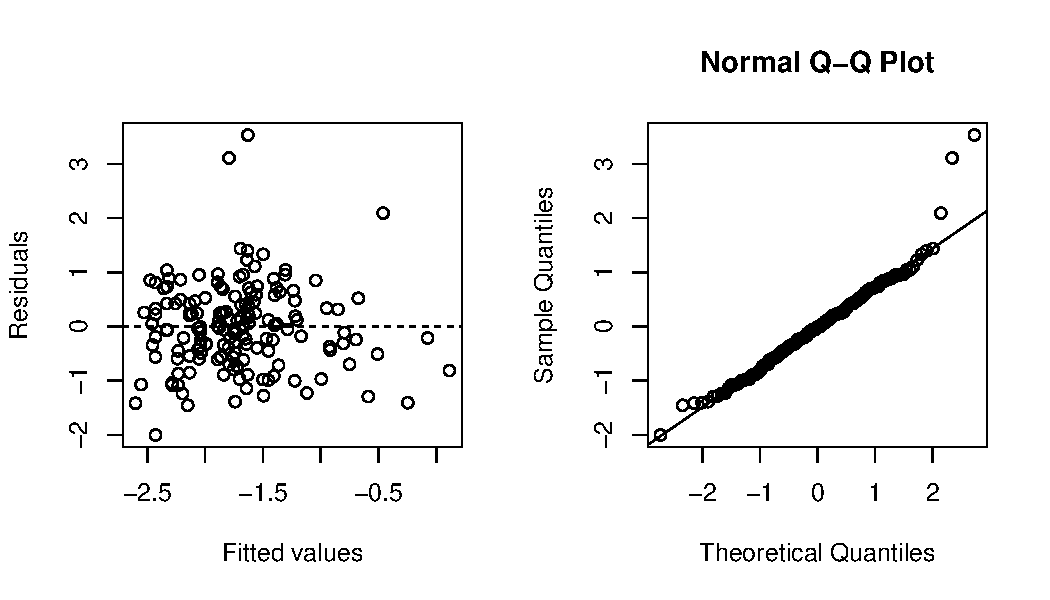
\includegraphics{Bio144_2017_week4-modelChecksHg}
}

\frame{\frametitle{Multiple vs.\ many single regressions}
Question: I find group-specific intercepts and interactions too complicated. Could I simply fit separate models for each group?\\[6mm]

\pause
Answer (Stahel 3.3o):\\[4mm]
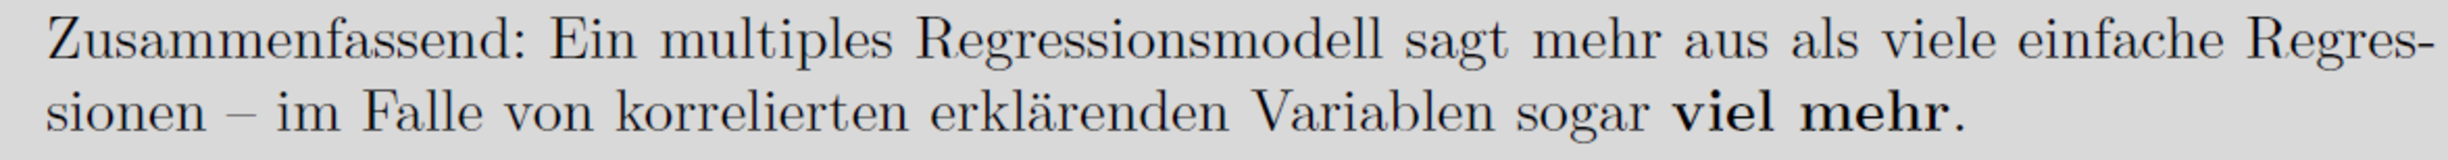
\includegraphics[width=11cm]{pictures/citation.pdf}
~\\[4mm]

Why?
}

\frame{\frametitle{}
Chapter 3.3c in the Stahel script illustrates the point on four artificial examples. The model is given as 
\begin{equation*}
y_i = \beta_0 + \beta_1 x_i^{(1)} + \beta_2 x_i^{(2)} + e_i \  ,
\end{equation*}

where $\bm{x}^{(1)}$ is a continuous variable, and  $\bm{x}^{(2)}$ is a binary grouping variable (0/1)
}
%\frame{References:
%\bibliographystyle{Chicago}
%\bibliography{refs}
%}

\end{document}
